\section{Background}
\label{sec:background}
We begin by providing a brief review of forecasting systems, followed by a
quick preview of EMBERS, its system architecture, machine learning models,
and measures for evaluating its performance. For more details, please
see~\cite{kdd:beating-the-news}.

Forecasting societal events such as civil unrest has a long tradition in the intelligence analysis and political science
community. We distinguish between forecasting systems versus event coding
%adding the extra 'systems' here keeps ICEWS+footnote from moving into margin
systems (systems that provide
structured representations of ongoing events reported in newspapers), and focus on the former.
Early forecasting systems such as ICEWS~\cite{icews} provided very broad coverage in countries but
were limited by their spatio-temporal resolution (e.g., typically country- and month- level forecasting for
specific events of interest~\cite{eoiprediction}). The ICEWS events of interest are
domestic political crises, international crises, ethnic/religious violence, insurgencies,
and rebellion.
A similar project in scope is PITF (Political Instability
Task Force)~\cite{pitf} funded by the CIA.
To the best of our knowledge, only EMBERS provides
the most-specific spatial resolution (city-level) and the most-specific
temporal resolution (daily-level) capability in forecasting.

The software architecture of EMBERS (Early Model Based Event Recognition using
Surrogates) is designed as a loosely coupled, share-nothing, highly distributed pipeline of
processes connected via ZeroMQ.  In this manner, the system is both highly scalable and fault
tolerant.  The EMBERS pipeline can loosely be broken up into four stages:
ingestion, enrichment, modeling, and selection.  In the first stage, ingestion,
data is collected from a variety of sources and streamed into the following
stages in real-time.  The enrichment stage takes the raw data from the ingestion stage
and processes it in various ways including natural language processing,
geocoding, and relative time phrase normalization.  After enrichment, the
modeling stage feeds the enriched data into the various models that make up
EMBERS.  Unlike other systems which use single monolithic models to make
predictions, EMBERS combines the results of several different models to arrive
at the most accurate forecasts.  In particular, the separate
alerts from each model are de-duplicated, fused, and selected and finally
emitted as a full forecast for a real world event.

\begin{figure}
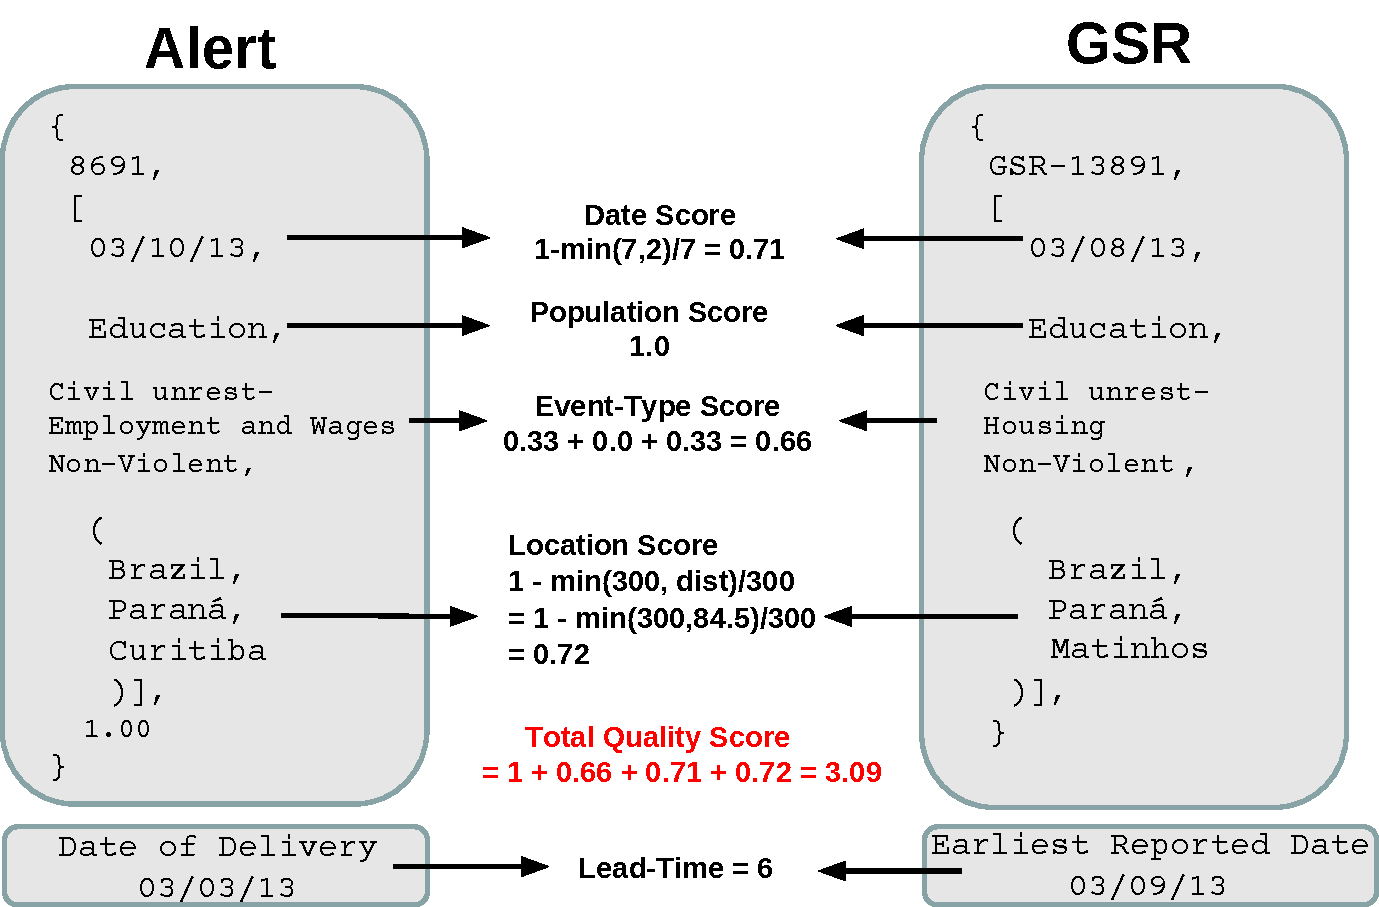
\includegraphics[width=\columnwidth]{figures/cu/alert_vs_gsr.pdf}
\caption{An example depicting how an alert is scored with respect to the ground truth.}
\label{fig:alert}
\end{figure}

The structure of a civil unrest forecast is shown in
Figure~\ref{fig:alert} (left).
A forecast constitutes four fields, corresponding to the when, where, who, and why
of the protest. These fields are respectively denoted as the date, location, population, and event type.
Location is recorded at the city level. Population and event type are fields chosen from a categorical
set of possibilities.  The figure further shows how an alert with all
these fields are scored against a GSR event. In the basic scoring
methodology shown in Figure~\ref{fig:alert} each of the four fields
are weighted uniformly and a total quality score out of 4 is
obtained.  Apart from this each alert also has a lead-time associated with
it calculated as shown in Figure~\ref{fig:leadtime}.

\begin{figure}
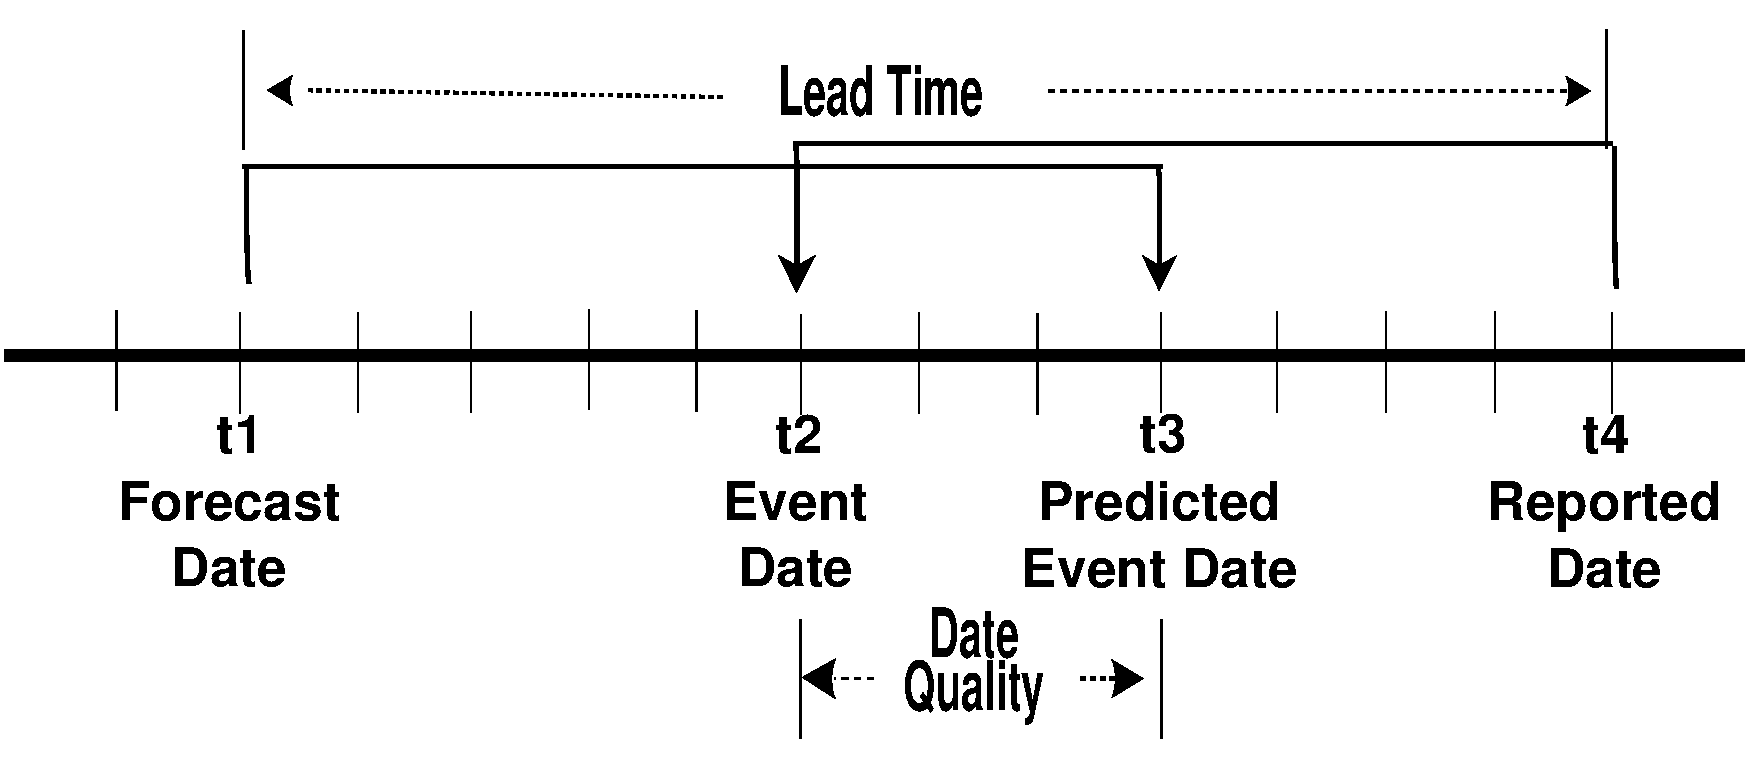
\includegraphics[width=\columnwidth]{figures/cu/timeline.pdf}
\caption{Alert sent at time $t1$ predicting an event at time $t3$
can be matched to a GSR event that happened at time $t2$ and reported
at time $t4$ if $t1 < t4$.}
\label{fig:leadtime}
\end{figure}

Rather than design one model to integrate all possible data sources, EMBERS adopted a multi-model
approach to forecasting. Each model utilized a specific (possibly overlapping) set of data sources
and is tuned for high precision, so that the union of these models can be tuned for high recall.
A fusion/suppression engine~\cite{andy-scotland-paper} allows a tunable
strategy to issue more or fewer
alerts depending on whether the analyst's objective is to obtain a higher
precision or recall. The underlying models used in EMBERS are: (i)
\textit{planned protest model}~\cite{pp-paper1},
(ii) \textit{dynamic query expansion}~\cite{dqe-plosone}, (iii) \textit{volume-based model}~\cite{asonam},
(iv) \textit{cascade regression}~\cite{anil-plosone}, and (v) a baseline model. The planned protest model,
for news and social media (Twitter, Facebook), identifies explicit signs of organization and calls
for protest, resolves relative mentions of time (e.g., `next Saturday') and space (e.g., `the square')
to issue forecasts. The dynamic query expansion (DQE) model uses Twitter as a data source and learns time- and country-specific
expansions of a seed set of keywords to identify specific situational circumstances for civil unrest.
For instance, in Venezuela (an economy where the government exercises stringent price controls),
there were a series of protests in 2014 stemming from the shortage of toilet paper, a novel circumstance
that was uncovered by DQE. The volume-based model uses a range of data sources, spanning
social, economic
and political indicators. It uses classical statistical models (LASSO
and hybrid regression models) to forecast civil unrest events using features
from social media (Twitter and blogs), news sources,
political event databases (ICEWS and GDELT~\cite{gdelt}), Tor~\cite{tor} statistics, food prices, and currency
exchange rates. It aims to provide a multi-source perspective into forecasting by leveraging
the selective superiorities of different data sources.  The cascade regression model
aims to model activity related to organization and mobilization in Twitter~\cite{anil-plosone}.
Finally, the baseline model uses maximum likelihood
estimation over the GSR to issue history-based forecasts.

The EMBERS project is unique not just in its algorithmic underpinnings but also in the use of new measures
for evaluation, specifically aimed at determining forecasting performance. As
shown in Figure~\ref{fig:leadtime},
one of the primary measures of EMBERS performance is lead time, the number of days by which a forecast
`beats the news', i.e., the date of reporting of the event. Lead time should not be confused with
date quality, i.e., the difference between the predicted date and the actual date of the event. The date
quality is one of the components of the quality score, the other components being the
location score, event type score, and population score.
Figure~\ref{fig:alert} 
shows how these other
components are scored between an EMBERS forecast and a GSR record.
\iffalse
{\color{red} Note
that in the event-type score 1/3 is given for identifying if the alert
is a civilunrest. Though this paper talks only about civilunrest events and
thus all alerts discussed here by default get 1/3 for the event-type score, the reason
for this is that the EMBERS system also made forecasts for other categories like ILI
(Influenza like Illness) counts, Rare disease (like hantavirus)
occurences etc. One-third of the event-type score was given to
identifying the category of event (civilunrest/ILI/rare disease)
correctly.}
\fi

Given a set of alerts and a set of
GSR events for a given month, the lead time is used as a constraint to define legal (alert, event) pairs so that
we can construct a bipartite matching to optimize the best quality
score. From this bipartite matching,
measures of precision and recall can be derived, i.e., by assessing the number of (un)matched events or
alerts. Finally, a confidence score is used to assess the quality of probabilities imputed by EMBERS to its
forecasts, and measured in terms of the Brier score. For more details, please
see~\cite{kdd:beating-the-news}.

We now turn to a discussion of specific discoveries enabled by EMBERS, into civil unrest in Latin America, and into
the complexity of the forecasting enterprise as a whole.

